\section{Pre-amplificatore}
	Il pre-amplificatore è realizzato dal circuito in
	\figurename{ \ref{fig:ampli}}.

		\begin{figure}[h]
		\begin{minipage}{0.75\textwidth}
			\centering
			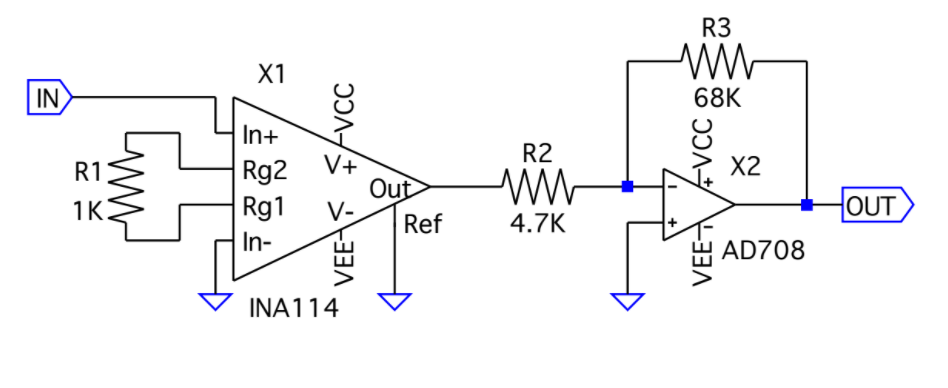
\includegraphics[width=\textwidth]{ampli.png}
			\caption{Circuito pre-amplificatore.}
			\label{fig:pre}
		\end{minipage}
		\begin{minipage}{0.19\textwidth}
			\begin{tabular}{l@{ }c@{ }l}
				$R_{1}$& = &\SI{0.971(9)}{\kilo\ohm}\\
				$R_{2}$& = &\SI{4.69(5)}{\kilo\ohm}\\
				$R_3$& = &\SI{71.9(7)}{\kilo\ohm}\\
			\end{tabular}
		\end{minipage}
	\end{figure}

	Essendo il guadagno atteso in $out$ $\sim 51 \cdot 14.5 \sim 740$, per effettuare
	la verifica evitando che l'uscita degli OpAmp saturi senza dover inviare segnali molto piccoli e dunque relativamente molto rumorosi
	si è scelto di valutare separatamente l'amplificazione delle due sezioni; è
	inoltre stato montato un partitore di tensione (impiegando le resistenze $R_{T1}=\SI{0.987(9)}{\kilo\ohm}$ e $R_{T2}=\SI{1031(9)}{\kilo\ohm}$) per valutare più agevolmente l'amplificazione della prima sezione.

	Si è proceduto pertanto ad inviare in ingresso al partitore un onda sinusoidale di varie ampiezze, misurando l'ampiezza dell'onda in uscita all'INA114.

	Il guadagno ottenuto $Av_{1}= 55 \pm 1$ risulta compatibile con le attese $\sim 51$.

	Effettuata questa prima verifica si è proceduto a verificare il guadagno della seconda
	parte del circuito montato.
	Essendo i due circuiti indipendenti si sono di nuovo inviati direttamente alla resistenza $R_2$ segnali sinusoidali generati esternamente anzichè collegarvi l'output del precedente OpAmp.

	Si è misurato un guadagno $Av_2=\num{15.50(1)}$, compatibile col valore atteso $\longfrac{R_3}{R_2} = \num{15.33(18)}$.


	\begin{figure}[h]
		\centering
		\subfloat[Prima sezione, INA114.]{
			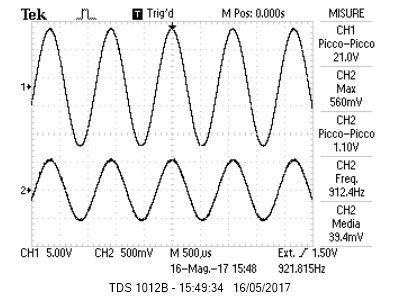
\includegraphics[scale=0.5]{preamp1.png}
		}
		\qquad
		\subfloat[Seconda sezione, AD708.]{
			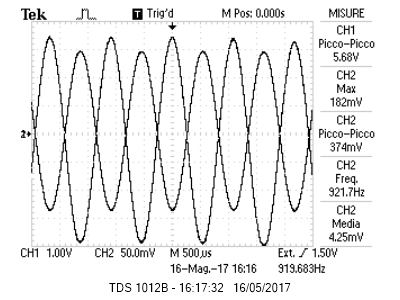
\includegraphics[scale=0.5]{preampb.png}
		}
		\caption{Acquisizioni esemplificative di segnali in ingresso (ch. 1) e in uscita (ch. 2).}
		\label{fig:preampo}
	\end{figure}
